\documentclass[11pt]{article}
\usepackage[a4paper,margin=0.85in]{geometry}
\usepackage[T1]{fontenc}
\usepackage[utf8]{inputenc}
\usepackage{lmodern}
\usepackage{microtype}
\usepackage{amsmath,amssymb}
\usepackage{array,booktabs,tabularx}
\usepackage{float}
\usepackage{xcolor}
\usepackage{tikz}
\usepackage[hidelinks]{hyperref}
\usepackage{url}

\usetikzlibrary{arrows.meta,positioning,shapes.geometric,calc,decorations.markings}

\setlength{\parindent}{0pt}
\setlength{\parskip}{5pt}
\emergencystretch=2em

\definecolor{constellationBlue}{HTML}{1F5FBF}
\definecolor{constellationInk}{HTML}{172033}
\definecolor{constellationGreen}{HTML}{1C7C62}
\definecolor{constellationRed}{HTML}{B42318}
\definecolor{constellationAmber}{HTML}{B7791F}
\definecolor{constellationSoft}{HTML}{F5F7FB}
\definecolor{constellationRule}{HTML}{D8DEE9}

\hypersetup{
  colorlinks=true,
  linkcolor=constellationBlue,
  citecolor=constellationBlue,
  urlcolor=constellationBlue,
  pdftitle={Question Constellation Research Paper},
  pdfauthor={Question Constellation Inc}
}

\newcolumntype{Y}{>{\raggedright\arraybackslash}X}
\newcolumntype{L}[1]{>{\raggedright\arraybackslash}p{#1}}

\newcommand{\paperkicker}[1]{%
  \begin{center}
    \small\textsc{#1}
  \end{center}
}

\newcommand{\affiliationblock}{%
  Question Constellation Inc
}

\newcommand{\keywords}[1]{%
  \vspace{0.5em}
  \noindent\textbf{Keywords:} #1
}

\newcommand{\claimbox}[2]{%
  \begin{center}
    \fcolorbox{constellationRule}{constellationSoft}{%
      \begin{minipage}{0.92\linewidth}
      \textbf{#1}\par
      #2
      \end{minipage}}
  \end{center}
}

\newcommand{\link}[2]{\href{#1}{#2}}
\newcommand{\sourcepath}[1]{\texttt{\detokenize{#1}}}
\newcommand{\chain}[1]{\texttt{\detokenize{#1}}}

\newcommand{\protocolbox}[2]{%
  \begin{center}
    \fcolorbox{constellationBlue}{constellationSoft}{%
      \begin{minipage}{0.9\linewidth}
      \textbf{#1}\par
      #2
      \end{minipage}}
  \end{center}
}

\tikzset{
  process/.style={
    rectangle,
    rounded corners=2pt,
    draw=constellationBlue,
    fill=constellationSoft,
    line width=0.7pt,
    minimum height=8mm,
    align=center,
    text width=28mm,
    font=\small
  },
  processWide/.style={
    rectangle,
    rounded corners=2pt,
    draw=constellationBlue,
    fill=constellationSoft,
    line width=0.7pt,
    minimum height=8mm,
    align=center,
    text width=40mm,
    font=\small
  },
  decision/.style={
    diamond,
    aspect=1.9,
    draw=constellationAmber,
    fill=constellationSoft,
    line width=0.7pt,
    align=center,
    text width=26mm,
    font=\small
  },
  arrow/.style={
    -{Latex[length=2.2mm]},
    line width=0.7pt,
    draw=constellationInk
  },
  midRetryArrow/.style={
    densely dashed,
    line width=0.7pt,
    draw=constellationAmber,
    postaction={decorate},
    decoration={
      markings,
      mark=at position 0.74 with {\arrow{Latex[length=2.2mm]}}
    }
  },
  chartbar/.style={
    draw=constellationBlue,
    fill=constellationBlue!18,
    line width=0.5pt
  }
}

\newcommand{\simplebar}[5]{%
  \draw[chartbar] (#1,0) rectangle ++(#3,#4);
  \node[below,align=center,font=\scriptsize,text width=22mm] at ($(#1,0)+(#3/2,0)$) {#2};
  \node[above,font=\scriptsize] at ($(#1,0)+(#3/2,#4)$) {#5};
}

\hypersetup{
  pdftitle={Question Constellation: Answer Chains for Repairable Exam Reasoning, Transfer Practice, and Learning Analytics},
  pdfauthor={Question Constellation Inc}
}

\title{\textbf{Question Constellation:\\Answer Chains for Repairable Exam Reasoning, Transfer Practice, and Learning Analytics}}
\author{\affiliationblock}
\date{17 July 2026}

\begin{document}
\maketitle

\begin{abstract}
Exam-practice systems commonly organize questions by subject, topic, paper, mark value, command word, or text similarity. Those categories are useful for retrieval, but they do not directly represent the ordered reasoning that earns marks, nor do they explain what a learner should repair after a weak answer. This paper investigates \textit{answer chains}: compact, mark-scheme-grounded sequences of reasoning links for diagnosing missing links, supporting rewrite feedback, generating stepping-stone practice, selecting transfer questions, and producing interpretable learning analytics.

The paper develops five connected components of the Question Constellation architecture. First, it formalizes answer chains as auditable representations of mark-scoring reasoning. Second, it specifies missing-link feedback, a feedback design that labels present, partial, and missing chain links before a learner rewrites and attempts a transfer question. Third, it defines stepping stones, small preparatory tasks generated from diagnosed exam failures to isolate and rehearse one missing operation before support is faded. Fourth, it introduces retained answer chains as a learner-facing analytics unit for tracking repair, transfer, delayed recall, recurrence, and confidence calibration. Fifth, it specifies the Missing-Link GCSE Benchmark, a dataset design that evaluates not only mark prediction but link-state detection, missing-link diagnosis, repair feedback, and transfer-question selection.

The current local corpus contains 16 extracted official-paper JSON artifacts and 503 extracted questions: 373 from AQA Combined Science materials and 130 from AQA Biology materials. We report two preliminary evaluations. A deterministic simulated-user harness over four guided-gap cases obtains 0.9559 link-state accuracy and 0.7647 primary-gap accuracy. A 48-run model-grading comparison over 16 GCSE answer fixtures finds expected-mark-range accuracy of 15/16 for \texttt{chatgpt-gpt-5.3-codex-spark}, 14/16 for \texttt{chatgpt-gpt-5.4-fast}, and 15/16 for \texttt{chatgpt-gpt-5.4-mini}. These results are not learner-outcome evidence; they instead motivate a benchmark agenda for evaluating repairable exam reasoning beyond mark prediction.
\end{abstract}

\keywords{educational technology; intelligent tutoring systems; automatic short-answer grading; formative feedback; learning analytics; benchmark datasets; GCSE; answer chains; transfer; interpretable AI}

\section{Introduction}

Most exam-practice products are good at retrieval. They help a learner find questions by board, paper, subject, topic, mark value, tier, or command word. Retrieval matters: students need questions that match their specification and exam context. But retrieval does not explain why a learner lost marks or what they should practise next. A student may filter correctly to GCSE Biology, circulation, four-mark explanation questions, and still omit the oxygen-to-respiration link that a mark scheme rewards. Another student may know a physics formula but skip the collision mechanism that connects particle motion to power transfer.

The central design problem is therefore not only \textit{find me another similar question}. It is:

\begin{center}
\chain{Which reusable missing link caused this weak answer, and where should the learner practise that link next?}
\end{center}

Question Constellation answers that question with answer chains. An answer chain is a compact, source-grounded sequence of links such as:

\begin{center}
\chain{reduced delivery -> less oxygen -> less aerobic respiration -> less energy or symptom}
\end{center}

The chain is not a topic label, a model answer, or a generated explanation. It is a small representation of the ordered reasoning that earns marks and can recur across surface-different questions. A topic says what content is involved. A chain says what the answer must connect.

\claimbox{Research questions}{RQ1: Can official exam questions and mark evidence be represented as compact answer chains that remain reusable across surface-different questions? RQ2: Can models and deterministic baselines detect link states and identify primary missing links with enough reliability to support feedback? RQ3: Which evaluation tasks are needed to test repair, transfer, and retained-chain review rather than mark prediction alone?}

This paper consolidates a representation, dataset, system, and evaluation agenda around those questions. It is also intentionally honest about evidence. The current implementation artifacts and adjacent project materials support a system specification, corpus description, preliminary model evaluation, benchmark design, and study protocols. They do not yet support claims about learner outcome gains.

\subsection{Contributions}

The paper makes eight contributions:

\begin{enumerate}
\item It defines the answer-chain representation for mark-scheme-grounded exam reasoning.
\item It specifies a two-phase extraction and chain-reconciliation pipeline that separates source fidelity from semantic chain grouping.
\item It designs missing-link feedback as an experimentally testable intervention.
\item It defines stepping stones as generated preparatory practice derived from diagnosed failures.
\item It proposes retained answer chains as an interpretable learning-analytics object.
\item It specifies a benchmark schema and task suite for repairable GCSE exam reasoning.
\item It reports a preliminary model-grading comparison across three currently available ChatGPT/Codex model variants.
\item It gives a staged evaluation roadmap that avoids overclaiming before learner data are collected.
\end{enumerate}

\section{System Overview}

Question Constellation should feel like a lightweight public GCSE question bank and exam-question atlas organized by answer chains. It should not start as a generic chatbot, a full learning workspace, or a dashboard-first revision app. The first-use loop is concrete:

\begin{center}
\chain{public question -> answer chain -> constellation -> practice -> transfer}
\end{center}

Runtime model use is optional and lightweight. Curated questions, model answers, mark checklists, common weak answers, static chain structure, and reviewed constellations should carry most product value. If a model is used, it should sit behind an explicit action such as \textit{Check answer}, and its output should be reduced to auditable link states and feedback targets.

\begin{figure}[H]
\centering
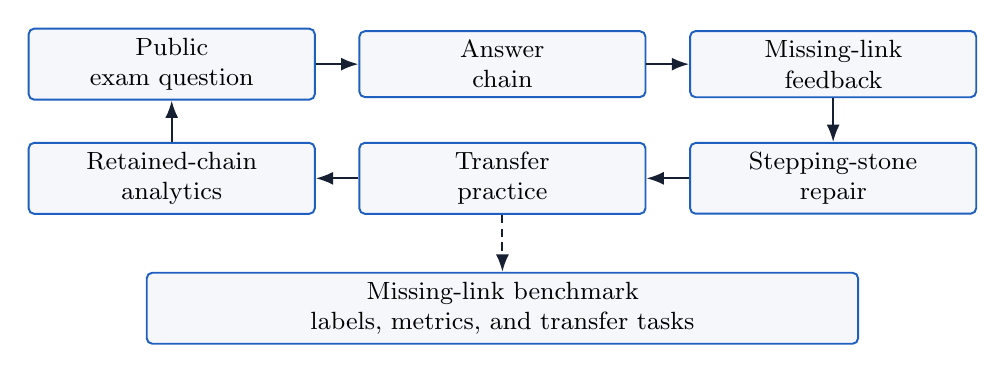
\begin{tikzpicture}
  \node[processWide,text width=34mm] (question) at (0,1.45) {Public\\exam question};
  \node[processWide,text width=34mm] (chain) at (4.2,1.45) {Answer\\chain};
  \node[processWide,text width=34mm] (feedback) at (8.4,1.45) {Missing-link\\feedback};
  \node[processWide,text width=34mm] (stones) at (8.4,0) {Stepping-stone\\repair};
  \node[processWide,text width=34mm] (transfer) at (4.2,0) {Transfer\\practice};
  \node[processWide,text width=34mm] (retained) at (0,0) {Retained-chain\\analytics};
  \node[processWide,text width=88mm] (benchmark) at (4.2,-1.65) {Missing-link benchmark\\labels, metrics, and transfer tasks};
  \draw[arrow] (question) -- (chain);
  \draw[arrow] (chain) -- (feedback);
  \draw[arrow] (feedback) -- (stones);
  \draw[arrow] (stones) -- (transfer);
  \draw[arrow] (transfer) -- (retained);
  \draw[arrow] (retained.north) -- (question.south);
  \draw[arrow,densely dashed] (transfer.south) -- (benchmark.north);
\end{tikzpicture}
\caption{Unified Question Constellation architecture. The benchmark evaluates the same objects used by the product loop.}
\label{fig:architecture}
\end{figure}

\section{Local Corpus and Source Grounding}

The local corpus used to ground the system design is concentrated in GCSE science. It contains 16 extracted official-paper JSON artifacts and 503 extracted questions, split into 373 AQA Combined Science questions and 130 AQA Biology questions. These counts were verified from \sourcepath{data/vision-extracted}. The semantic-chain artifacts include answer-chain candidates, constellation candidates, supporting questions, transfer-distance labels, review flags, evidence summaries, demoted candidates, and excluded-neighbor notes.

\begin{figure}[H]
\centering
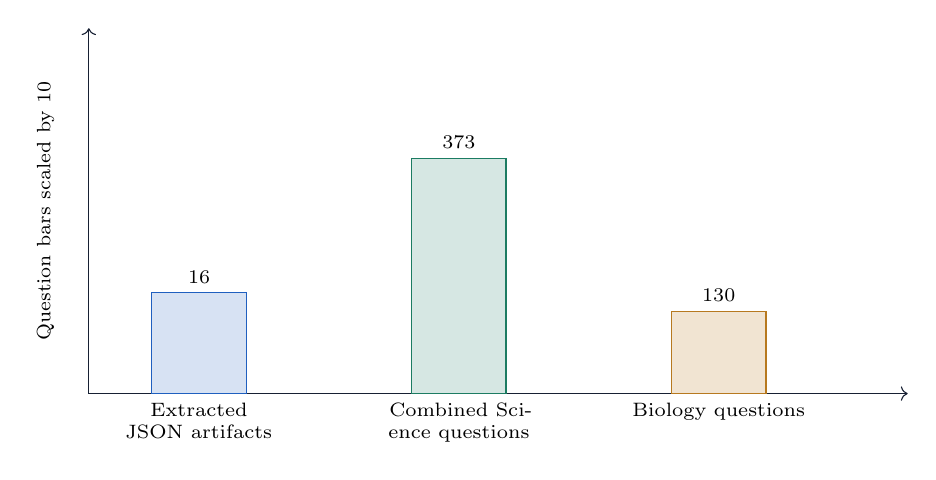
\begin{tikzpicture}[x=1cm,y=0.08cm]
  \draw[->,draw=constellationInk] (0,0) -- (10.4,0);
  \draw[->,draw=constellationInk] (0,0) -- (0,58);
  \draw[chartbar] (0.8,0) rectangle (2.0,16);
  \node[below,align=center,font=\scriptsize,text width=24mm] at (1.4,0) {Extracted JSON artifacts};
  \node[above,font=\scriptsize] at (1.4,16) {16};
  \draw[chartbar,fill=constellationGreen!18,draw=constellationGreen] (4.1,0) rectangle (5.3,37.3);
  \node[below,align=center,font=\scriptsize,text width=26mm] at (4.7,0) {Combined Science questions};
  \node[above,font=\scriptsize] at (4.7,37.3) {373};
  \draw[chartbar,fill=constellationAmber!20,draw=constellationAmber] (7.4,0) rectangle (8.6,13);
  \node[below,align=center,font=\scriptsize,text width=24mm] at (8.0,0) {Biology questions};
  \node[above,font=\scriptsize] at (8.0,13) {130};
  \node[rotate=90,font=\scriptsize] at (-0.55,29) {Question bars scaled by 10};
\end{tikzpicture}
\caption{Local source corpus used for representation and system design.}
\label{fig:corpus}
\end{figure}

The corpus is not a student-response benchmark. It does not support claims about effect sizes, retention gains, or transfer improvement. It supports a different kind of evidence: whether official questions, mark schemes, checklists, model answers, and chain memberships can be extracted, audited, and organized into reusable repair objects.

Spark guided-gap flows provide local design cases for manual missing-link repair:

\begin{itemize}
\item particle collisions and power;
\item alpha-scattering evidence;
\item circuit adjustment method;
\item coronary artery causal chain.
\end{itemize}

These flows are examples of the desired interaction pattern. They show a weak answer, diagnose a gap, ask builder questions, display a repaired chain, and compose an improved answer. They are not outcome data.

\begin{table}[H]
\centering
\small
\begin{tabularx}{\linewidth}{L{0.22\linewidth}Y Y}
\toprule
\textbf{Design case} & \textbf{Observed weak-answer gap} & \textbf{Repair operation}\\
\midrule
Particle collisions and power & Learner jumps from faster particles to higher power. & Insert more frequent or harder collisions with turbine blades before energy per second.\\
Alpha scattering evidence & Learner recalls models but does not connect observations to conclusions. & Pair each experimental result with the atomic-structure conclusion it supports.\\
Circuit adjustment method & Learner identifies reversing connections but misses smooth control. & Replace battery swapping with a variable resistor and repeat after reversing connections.\\
Coronary artery chain & Learner starts with reduced blood flow but stops before the cell-process mechanism. & Add oxygen, aerobic respiration, energy release, and symptom or impaired function.\\
\bottomrule
\end{tabularx}
\caption{Local guided-gap design cases from Spark. These are workflow examples, not outcome evidence.}
\label{tab:designcases}
\end{table}

\section{Related Work}

\subsection{Automatic short-answer grading and educational NLP}

Automatic short-answer grading has a long history. Burrows, Gurevych, and Stein review eras and trends in automatic short-answer grading and emphasize the importance of comparable evaluation \cite{burrows2015}. Mohler, Bunescu, and Mihalcea model short-answer grading using semantic similarity and dependency graph alignment \cite{mohler2011}. SemEval-2013 Student Response Analysis frames student-answer evaluation as a recognition and semantic analysis problem \cite{dzikovska2013}. Recent LLM work extends this tradition: Latif et al. study knowledge distillation for science assessment scoring \cite{latif2023}, and Medly evaluates LLM performance on a real double-marked GCSE benchmark \cite{fox2026}.

These works ask whether a system can agree with human marks or labels. Question Constellation accepts that as a necessary capability but asks a downstream instructional question: after a score or checklist analysis exists, what should the learner practise next? A model can predict a correct mark and still fail to identify the repairable missing link.

\subsection{Multimodal and handwritten assessment}

Real exams often include handwriting, diagrams, formulae, source images, and layout-dependent response surfaces. Caraeni, Scarlatos, and Lan evaluate GPT-4 on handwritten mathematical solutions \cite{caraeni2024}. Kortemeyer, Nohl, and Onishchuk examine AI-assisted grading for handwritten thermodynamics exams \cite{kortemeyer2024}. These studies reinforce a key architectural decision: extraction and scoring reliability must be separated from the pedagogical representation. Answer chains are not a substitute for reliable extraction. They are built after prompts, assets, and mark evidence have been recovered.

\subsection{Feedback, tutoring, and transfer}

Feedback research distinguishes actionable feedback from simple scores. Hattie and Timperley analyze feedback as information that closes the gap between current and desired performance \cite{hattie2007}. Shute emphasizes formative feedback that is specific, timely, and task-focused \cite{shute2008}. Retrieval-practice work shows that producing answers and retrieving knowledge can improve retention \cite{roediger2006}, and Butler's transfer work suggests that repeated testing can improve application to new questions \cite{butler2010}. Karpicke and Blunt further show that retrieval practice can outperform elaborative studying with concept mapping \cite{karpicke2011}.

Question Constellation operationalizes the retrieved object as an answer chain. The learner should not merely reread a model answer. They should reconstruct the missing link and use it on a different question.

\subsection{Knowledge tracing and learning analytics}

Bayesian Knowledge Tracing models acquisition of procedural knowledge as latent skill mastery \cite{corbett1994}. Learning Factors Analysis provides a method for evaluating and improving cognitive models \cite{cen2006}. Deep Knowledge Tracing uses neural sequence models to predict learner performance \cite{piech2015}. Intelligent tutoring systems show meaningful effects in meta-analysis \cite{kulik2016}, while recent human-AI tutoring work such as Tutor CoPilot explores how AI can guide tutors in real time \cite{wang2024}.

These methods require skill units. Answer chains are proposed as a transparent skill unit for exam reasoning: small enough to diagnose a link, broad enough to transfer, and visible enough for learners and teachers.

\subsection{Scaffolding, worked examples, and assistance}

Stepping-stone practice is motivated by scaffolding and cognitive-load research. Wood, Bruner, and Ross describe tutoring support that enables learners to solve problems beyond unaided performance \cite{wood1976}. Sweller's cognitive-load theory explains why full exam problems can overwhelm learners before the relevant schema is stable \cite{sweller1988}. Worked-example research shows the value of guided examples when learners are not yet ready for full problem solving \cite{renkl2002}. Koedinger and Aleven describe the assistance dilemma: learners can receive too much help or too little \cite{koedinger2007}. Stepping stones address that dilemma by training the missing link and fading support.

\section{Answer Chains}

\subsection{Definition}

An answer chain is a compact ordered sequence of mark-scoring links. It is both student-facing and evidence-grounded. The object has the fields in Table~\ref{tab:chainfields}.

\begin{table}[H]
\centering
\small
\begin{tabularx}{\linewidth}{L{0.24\linewidth}Y}
\toprule
\textbf{Field} & \textbf{Function}\\
\midrule
Title & Short learner-facing handle.\\
Canonical chain & Two to five compact links joined by arrows.\\
Step list & Ordered links with roles such as cause, process, method, evidence, or conclusion.\\
Mark evidence & Source mark-scheme items supporting each step.\\
Common omission & Weak-answer pattern the chain repairs.\\
Membership & Questions using the chain, with fit notes and transfer-distance labels.\\
Near misses & Similar-looking questions excluded because the mark-scoring logic differs.\\
\bottomrule
\end{tabularx}
\caption{Core answer-chain fields.}
\label{tab:chainfields}
\end{table}

The chain should be short enough to act as a memory handle. It should not become a paragraph, a full model answer, or a worked calculation. For a calculation question, a reusable chain may be:

\begin{center}
\chain{convert units -> substitute formula -> calculate -> correct unit}
\end{center}

The question's actual values and final numeric answer belong in the model answer and mark evidence, not the chain.

\subsection{Depth of abstraction}

The representation must sit at the right depth. A broad topic is too weak; it cannot identify the missing link. A copied answer is too narrow; it cannot transfer. Figure~\ref{fig:abstraction} shows the desired middle layer.

\begin{figure}[H]
\centering
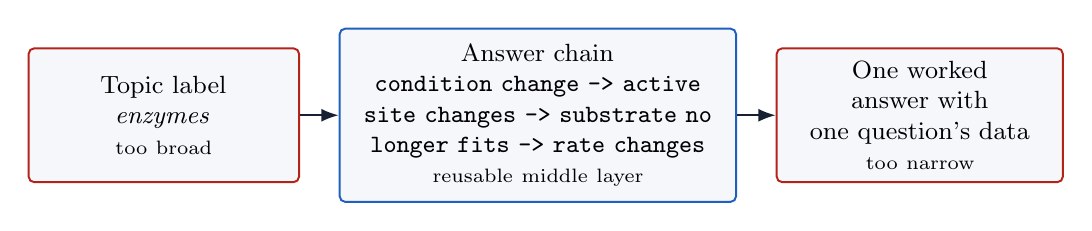
\begin{tikzpicture}
  \node[processWide,draw=constellationRed,text width=32mm,minimum height=17mm] (topic) at (0,0) {Topic label\\\textit{enzymes}\\{\scriptsize too broad}};
  \node[processWide,text width=48mm,minimum height=22mm] (chain) at (4.75,0) {Answer chain\\\chain{condition change -> active site changes -> substrate no longer fits -> rate changes}\\{\scriptsize reusable middle layer}};
  \node[processWide,draw=constellationRed,text width=34mm,minimum height=17mm] (answer) at (9.6,0) {One worked\\answer with\\one question's data\\{\scriptsize too narrow}};
  \draw[arrow] (topic.east) -- (chain.west);
  \draw[arrow] (chain.east) -- (answer.west);
\end{tikzpicture}
\caption{Answer chains occupy the middle layer between broad topics and one-question worked answers.}
\label{fig:abstraction}
\end{figure}

The cluster mechanism should therefore use this acceptance rule:

\protocolbox{Answer-chain acceptance rule}{%
Publish a learner-facing chain only when the same ordered links can repair the same kind of weak answer across real questions, every link has mark-scheme evidence or a documented variant, and plausible near misses have been excluded.}

\subsection{Data model}

In a database-backed product, answer chains sit alongside questions, mark-scheme items, checklists, model answers, and chain memberships:

\begin{itemize}
\item \texttt{questions}: prompt, metadata, mark value, page ranges, review flags;
\item \texttt{mark\_scheme\_items}: positive mark evidence and source guidance;
\item \texttt{mark\_checklist\_items}: learner-facing checklist items linked to mark evidence;
\item \texttt{model\_answers}: concise source-grounded model answers;
\item \texttt{answer\_chains}: canonical chain, title, subject, status, confidence;
\item \texttt{answer\_chain\_steps}: ordered links, roles, common omissions, evidence;
\item \texttt{question\_answer\_chains}: membership, transfer distance, fit notes.
\end{itemize}

The current app intentionally uses generated server-side data in local development, while D1 and R2 bindings are expected for deployed public data. The research argument does not depend on runtime model calls; it depends on the persistence of the chain object and its evidence.

\section{Extraction and Chain Reconciliation}

Question Constellation uses a two-phase pipeline. Source extraction comes first. Chain derivation comes second.

\begin{figure}[H]
\centering
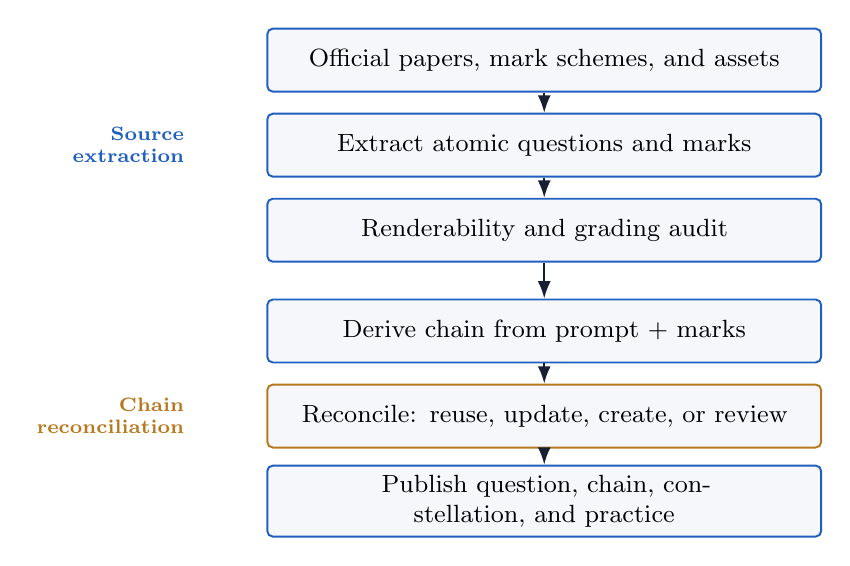
\begin{tikzpicture}
  \node[processWide,text width=68mm] (pdf) at (0,0) {Official papers, mark schemes, and assets};
  \node[processWide,text width=68mm] (extract) at (0,-1.08) {Extract atomic questions and marks};
  \node[processWide,text width=68mm] (audit) at (0,-2.16) {Renderability and grading audit};
  \node[processWide,text width=68mm] (chain) at (0,-3.44) {Derive chain from prompt + marks};
  \node[processWide,text width=68mm,draw=constellationAmber] (reuse) at (0,-4.52) {Reconcile: reuse, update, create, or review};
  \node[processWide,text width=68mm] (publish) at (0,-5.60) {Publish question, chain, constellation, and practice};
  \node[anchor=east,align=right,font=\scriptsize\bfseries,text=constellationBlue] at (-4.45,-1.08) {Source\\extraction};
  \node[anchor=east,align=right,font=\scriptsize\bfseries,text=constellationAmber] at (-4.45,-4.52) {Chain\\reconciliation};
  \draw[arrow] (pdf) -- (extract);
  \draw[arrow] (extract) -- (audit);
  \draw[arrow] (audit) -- (chain);
  \draw[arrow] (chain) -- (reuse);
  \draw[arrow] (reuse) -- (publish);
\end{tikzpicture}
\caption{Two-phase extraction and answer-chain reconciliation.}
\label{fig:pipeline}
\end{figure}

The separation matters. PDF extraction is a source-fidelity problem: recover page context, diagrams, response controls, formulae, answer-line structure, and mark-scheme evidence. Chain derivation is a semantic grouping problem over already extracted text and mark evidence. Mixing the two encourages premature chains before the source object is reliable.

\subsection{Chain reconciliation decisions}

For each extracted question, the chain phase should choose one of four decisions:

\begin{itemize}
\item \texttt{reuse\_existing}: the existing chain's ordered links fit the question;
\item \texttt{update\_existing}: the chain can be safely generalized after checking existing members;
\item \texttt{create\_new}: no existing chain fits and the new chain has evidence;
\item \texttt{needs\_review}: evidence is incomplete, ambiguous, or too one-off.
\end{itemize}

The system should not create a new chain merely because the paper, organism, object, command word, or mark value changes. It should compare ordered mark-scoring links and common weak-answer repairs.

\section{LLM Use, Guardrails, and Failure Modes}

Large language models can help build and operate Question Constellation, but they should not be the product's main source of value. The durable product objects should be extracted questions, mark-scheme items, checklists, model answers, answer chains, constellation memberships, retained-chain events, and benchmark labels. LLMs are best treated as bounded workers that propose or check those objects under evidence constraints.

\subsection{LLM roles}

\begin{table}[H]
\centering
\small
\begin{tabularx}{\linewidth}{L{0.23\linewidth}Y Y}
\toprule
\textbf{Role} & \textbf{Allowed output} & \textbf{Not allowed}\\
\midrule
PDF extraction assistant & Structured question, asset, response-control, mark-scheme, checklist, and provenance fields. & Creating reusable chains before source extraction is audited.\\
Chain reconciler & Reuse, update, create, or review decision with compact chain text and evidence links. & Grouping by topic, keywords, command word, or surface similarity alone.\\
Response checker & Link-state vector, evidence spans, primary missing link, and confidence. & Opaque chat feedback or unsupported marks.\\
Feedback planner & Short repair instruction tied to a missing link. & Revealing the full model answer before an attempt or inventing examiner authority.\\
Stepping-stone generator & Candidate micro-practice items with target link, expected response, feedback rule, and fade condition. & Generic easy worksheets not tied to the diagnosed link.\\
Benchmark pre-annotator & Draft labels for human review. & Final benchmark labels without adjudication.\\
\bottomrule
\end{tabularx}
\caption{Bounded LLM roles in Question Constellation.}
\label{tab:llmroles}
\end{table}

This division keeps runtime model use optional. A public question page, answer-chain page, and constellation page can work from reviewed static content. Model calls become useful behind explicit actions such as checking an answer, generating a repair candidate, or pre-annotating benchmark rows.

\subsection{Prompting protocol}

Every LLM prompt should follow five rules.

\begin{enumerate}
\item \textbf{Source first.} The model receives the prompt, mark scheme, chain, checklist, and allowed evidence. It should not infer source facts that are not present.
\item \textbf{Structured output.} The model returns JSON or another schema-bound object, not prose as the only artifact.
\item \textbf{Evidence fields.} Each chain step, checklist item, or link-state decision should cite source evidence or an answer span where possible.
\item \textbf{Abstention.} The model can choose \texttt{needs\_review}, \texttt{uncertain}, or \texttt{not\_enough\_evidence}; it should not force a confident label.
\item \textbf{No hidden authority.} The system should present model output as practice feedback unless a human-reviewed mark is available.
\end{enumerate}

The prompt templates in Appendix~\ref{appendix:prompts} instantiate this protocol.

\subsection{LLM failure modes}

\begin{table}[H]
\centering
\small
\begin{tabularx}{\linewidth}{L{0.24\linewidth}Y Y}
\toprule
\textbf{Failure mode} & \textbf{Example} & \textbf{Mitigation}\\
\midrule
Hallucinated mark evidence & Model invents a marking point not in the scheme. & Require source item ids and fail missing evidence.\\
Over-broad chain & \chain{cause -> process -> effect}. & Enforce compact but domain-specific chain text and near-miss review.\\
Over-specific chain & Chain includes one question's numeric substitution. & Run specificity audit and keep numbers in model answers.\\
Feedback leakage & Model gives full answer instead of repair prompt. & Use condition-specific templates and check for model-answer copying.\\
Prompt injection from answer & Student text says to ignore rubric. & Treat student answer as quoted data; never as instructions.\\
Overconfident scoring & Model gives a mark despite uncertain evidence. & Store confidence and allow abstention/review.\\
Model drift & Same prompt changes behavior after model update. & Version prompts, model ids, and feedback artifacts.\\
Equity and language bias & Nonstandard phrasing is marked missing despite correct reasoning. & Evaluate across paraphrases, dialect, and spelling variation with human review.\\
\bottomrule
\end{tabularx}
\caption{LLM failure modes and mitigations.}
\label{tab:llmfailures}
\end{table}

\subsection{Runtime architecture}

At runtime, the safest design is a retrieval-plus-structured-check pipeline. The app retrieves the reviewed question, answer chain, mark checklist, and model answer. The learner submits an attempt. The checker prompt receives only the relevant question package and the quoted answer. The model returns link states, evidence spans, a primary missing link, and a short repair target. A deterministic renderer then displays feedback in the product voice. This avoids letting the model improvise the full UI response.

For research, the same checker can be run offline against benchmark episodes. The LLM output should be evaluated separately on mark prediction, link-state detection, primary-gap diagnosis, repair-feedback quality, and transfer selection. A model that scores well on marks but poorly on primary-gap diagnosis is not sufficient for Question Constellation.

\section{Constellations and Transfer Ladders}

A constellation is a curated set of questions that use the same answer chain. The transfer ladder is:

\begin{center}
\chain{start -> near -> stretch -> exam transfer}
\end{center}

The start question is the clearest example. Near questions preserve the same chain with little surface change. Stretch questions move the chain into a less obvious context. Exam-transfer questions preserve the hidden chain in a more demanding exam-style setting.

Near misses are essential. A Biology question about statins or stents may share the circulation topic with a blood-flow chain, but it may not require the oxygen-to-respiration-to-energy reasoning. A Physics terminal-velocity question may share the word \textit{drag}, but the required chain may differ if the mark scheme focuses on resultant force rather than energy transfer. The system should name these exclusions so the constellation does not drift into topic clustering.

\begin{table}[H]
\centering
\small
\begin{tabularx}{\linewidth}{L{0.26\linewidth}Y}
\toprule
\textbf{Acceptance test} & \textbf{Publishable constellation requirement}\\
\midrule
Same weak answer & One specific weak-answer pattern explains common failure across the set.\\
Same repair & The same repair instruction improves answers across member questions.\\
Transfer ladder & The set has a clear start, near, stretch, and exam-transfer path where possible.\\
Excluded neighbor & Similar but invalid questions are named and excluded with reasons.\\
Memory sentence & The learner can retain the chain as one plain sentence.\\
Evidence support & Each visible link has mark-scheme support or remains review-gated.\\
Practice loop & The set supports attempt, diagnose, rewrite, transfer, and review.\\
\bottomrule
\end{tabularx}
\caption{Acceptance tests for learner-facing constellations.}
\label{tab:acceptance}
\end{table}

\section{Missing-Link Feedback}

\subsection{Intervention logic}

Missing-link feedback decomposes a learner's answer into chain-link states:

\begin{center}
\chain{present -> partial -> missing -> not required}
\end{center}

The feedback should identify the primary missing link, guide a rewrite, and then assign a transfer question. The intended learning loop is shown in Figure~\ref{fig:feedbackloop}.

\begin{figure}[H]
\centering
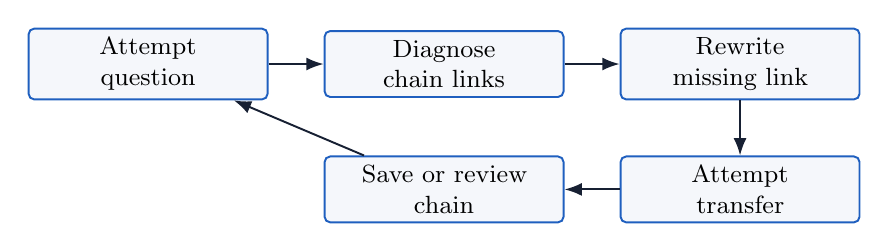
\begin{tikzpicture}[node distance=7mm]
  \node[process] (attempt) {Attempt\\question};
  \node[process,right=of attempt] (diagnose) {Diagnose\\chain links};
  \node[process,right=of diagnose] (repair) {Rewrite\\missing link};
  \node[process,below=of repair] (transfer) {Attempt\\transfer};
  \node[process,left=of transfer] (retain) {Save or review\\chain};
  \draw[arrow] (attempt) -- (diagnose);
  \draw[arrow] (diagnose) -- (repair);
  \draw[arrow] (repair) -- (transfer);
  \draw[arrow] (transfer) -- (retain);
  \draw[arrow] (retain) -- (attempt);
\end{tikzpicture}
\caption{Missing-link feedback loop.}
\label{fig:feedbackloop}
\end{figure}

The key outcome is not whether the learner can copy a model answer. The key outcome is whether the learner can use the repaired link in a different question.

\subsection{Study protocol}

A clean study compares three active feedback conditions:

\begin{table}[H]
\centering
\small
\begin{tabularx}{\linewidth}{L{0.24\linewidth}Y Y}
\toprule
\textbf{Condition} & \textbf{Learner sees after initial attempt} & \textbf{Instructional hypothesis}\\
\midrule
Model answer & Full model answer and total mark. & Helps same-question correction, but may encourage copying.\\
Mark checklist & Atomic checklist of credited points, with found and missing items. & Gives source-grounded requirements but may not name the reusable chain.\\
Missing-link feedback & Present/missing chain links, primary gap, short repair prompt, rewrite task, and transfer question. & Improves transfer by naming and rebuilding the reusable missing link.\\
\bottomrule
\end{tabularx}
\caption{Experimental conditions for missing-link feedback.}
\label{tab:feedbackconditions}
\end{table}

The primary outcome should be transfer performance on a different question using the same chain. Secondary outcomes include same-question rewrite gain, delayed chain recall, recurrence of the same missing link, time on task, and confidence calibration. The sample size should be determined by a power analysis before data collection. This manuscript does not invent a sample size.

\subsection{Instrumentation}

\begin{table}[H]
\centering
\small
\begin{tabularx}{\linewidth}{L{0.30\linewidth}Y}
\toprule
\textbf{Event} & \textbf{Required information}\\
\midrule
\texttt{initial\_answer\_submitted} & Learner id, session id, question id, chain id, answer pointer, timestamp.\\
\texttt{feedback\_shown} & Condition, mark, link-state vector, primary missing link, feedback version.\\
\texttt{rewrite\_submitted} & Rewrite pointer, link-state vector, repair gain, elapsed time.\\
\texttt{transfer\_answer\_submitted} & Transfer question id, mark, link-state vector, repeated missing link flag, confidence.\\
\texttt{delayed\_review\_submitted} & Delay interval, chain reconstruction score, transfer mark.\\
\bottomrule
\end{tabularx}
\caption{Minimum instrumentation for a missing-link feedback study. Raw answers should be stored separately from event metadata.}
\label{tab:feedbackevents}
\end{table}

\begin{table}[H]
\centering
\small
\begin{tabularx}{\linewidth}{L{0.26\linewidth}Y}
\toprule
\textbf{Threat} & \textbf{Mitigation}\\
\midrule
Model-answer copying & Use transfer performance as the primary outcome, not same-question rewrite alone.\\
Unequal question difficulty & Use matched chain sets and include question or chain effects in the model.\\
Feedback contamination & Randomize at session or class level when learners interact.\\
LLM variability & Store feedback version, model version where used, and deterministic checklist fallback.\\
Missing or partial responses & Predefine exclusion, imputation, and sensitivity rules.\\
Weak chain membership & Review study items before launch and exclude unresolved chain candidates.\\
\bottomrule
\end{tabularx}
\caption{Validity threats for a missing-link feedback experiment.}
\label{tab:validitythreats}
\end{table}

\section{Stepping-Stone Repair}

\subsection{Definition}

Some failures require a smaller task before the learner can retry. A stepping stone is a micro-practice item that isolates one missing chain link or prerequisite operation. It is not a hint on the original question and not a generic easier worksheet.

A valid stepping stone has five properties:

\begin{enumerate}
\item It targets one diagnosed link or operation.
\item It simplifies surface complexity while preserving the target reasoning.
\item It asks the learner to produce an answer.
\item It can be checked as present, partial, or missing.
\item It fades support before returning to transfer.
\end{enumerate}

\subsection{Generation pipeline}

\begin{figure}[H]
\centering
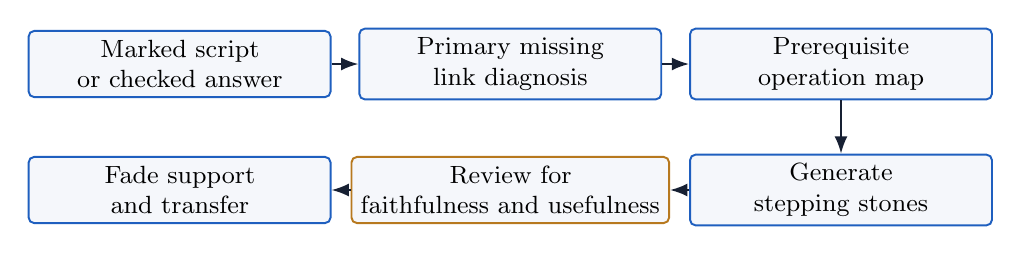
\begin{tikzpicture}
  \node[processWide,text width=36mm] (script) at (0,1.35) {Marked script\\or checked answer};
  \node[processWide,text width=36mm] (gap) at (4.2,1.35) {Primary missing\\link diagnosis};
  \node[processWide,text width=36mm] (pre) at (8.4,1.35) {Prerequisite\\operation map};
  \node[processWide,text width=36mm] (stone) at (8.4,-0.25) {Generate\\stepping stones};
  \node[processWide,text width=38mm,draw=constellationAmber] (review) at (4.2,-0.25) {Review for\\faithfulness and usefulness};
  \node[processWide,text width=36mm] (transfer) at (0,-0.25) {Fade support\\and transfer};
  \draw[arrow] (script) -- (gap);
  \draw[arrow] (gap) -- (pre);
  \draw[arrow] (pre) -- (stone);
  \draw[arrow] (stone) -- (review);
  \draw[arrow] (review) -- (transfer);
\end{tikzpicture}
\caption{Stepping-stone generation pipeline.}
\label{fig:stonespipeline}
\end{figure}

For the particle-collision case, a valid stepping stone asks what faster particles do to turbine blades and how that changes energy transfer per second. An invalid stepping stone merely asks for \(P=E/t\), because the missing link is not formula recall. For the alpha-scattering case, a valid stepping stone pairs each observation with its conclusion: most particles passing through suggests empty space; rare large deflections suggest concentrated positive charge and mass.

\subsection{Fading}

Fading is the mechanism that prevents stepping stones from becoming another form of answer leakage. The first item may expose the target link in a worked or highly constrained form, but later items should remove labels, sentence starters, and choice sets before the learner returns to a transfer question. The key design question is not whether the learner can complete an easier item once; it is whether support can be withdrawn while the same chain link remains intact.

\begin{figure}[H]
\centering
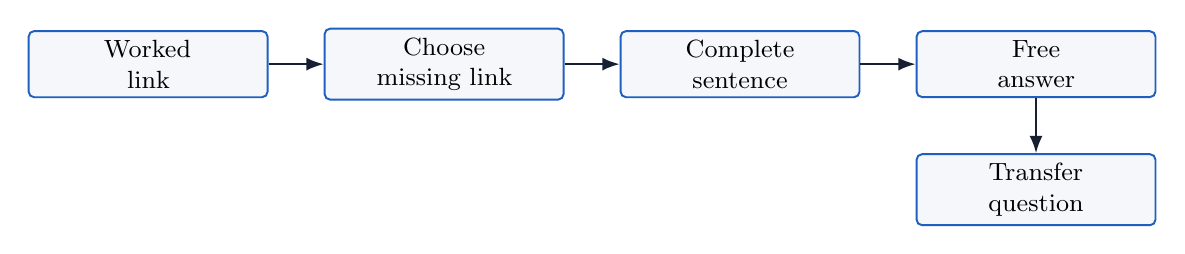
\begin{tikzpicture}[node distance=7mm]
  \node[process] (worked) {Worked\\link};
  \node[process,right=of worked] (choice) {Choose\\missing link};
  \node[process,right=of choice] (complete) {Complete\\sentence};
  \node[process,right=of complete] (free) {Free\\answer};
  \node[process,below=of free] (transfer) {Transfer\\question};
  \draw[arrow] (worked) -- (choice);
  \draw[arrow] (choice) -- (complete);
  \draw[arrow] (complete) -- (free);
  \draw[arrow] (free) -- (transfer);
\end{tikzpicture}
\caption{Support-fading ladder for a single missing link.}
\label{fig:fading}
\end{figure}

Operationally, the product should record the support level attached to every stepping stone. A transfer attempt is only interpretable if the system knows whether the learner reached it after a worked example, after a partial sentence, or after an independent short answer. This also gives the benchmark a way to distinguish direct feedback from scaffolded repair.

\subsection{Review rubric}

The review rubric treats generated stepping stones as draft instructional objects. A model may propose items, but a deployable item should pass checks for chain fidelity, cognitive-load reduction, clarity, feedback specificity, fading order, and transfer validity. Low scores should keep the item out of learner-facing practice rather than being hidden as model uncertainty.

\begin{table}[H]
\centering
\small
\begin{tabularx}{\linewidth}{L{0.27\linewidth}Y L{0.16\linewidth}}
\toprule
\textbf{Criterion} & \textbf{Reviewer question} & \textbf{Scale}\\
\midrule
Link fidelity & Does the item train the diagnosed missing link? & 0--3\\
Cognitive-load reduction & Is irrelevant load reduced without losing the target? & 0--3\\
Prompt clarity & Can a GCSE learner understand what to do? & 0--3\\
Feedback specificity & Can the answer be checked as present, partial, or missing? & 0--3\\
Fading order & Does the sequence reduce support coherently? & 0--3\\
Transfer validity & Does the final transfer preserve the same chain? & 0--3\\
\bottomrule
\end{tabularx}
\caption{Human review rubric for stepping stones.}
\label{tab:stonerubric}
\end{table}

This rubric is intentionally small enough for repeated use during dataset construction. It supports both product review and research annotation: reviewers can reject generic worksheets, flag items that solve the original question too directly, and preserve only those stepping stones that train the diagnosed operation.

\section{Retained Answer Chains}

\subsection{Rationale}

Learning analytics often tracks topics, scores, streaks, or completion. These signals are easy to display but weakly tied to transfer. A retained answer chain is a more interpretable object: a learner has seen, attempted, repaired, transferred, and possibly reviewed a specific mark-scoring chain.

The visible state should be earned. The current product should not expose the old standalone \sourcepath{/thinking-memory} route. Retained-chain review should be rebuilt only after practice produces meaningful chain history.

\subsection{State machine}

\begin{figure}[H]
\centering
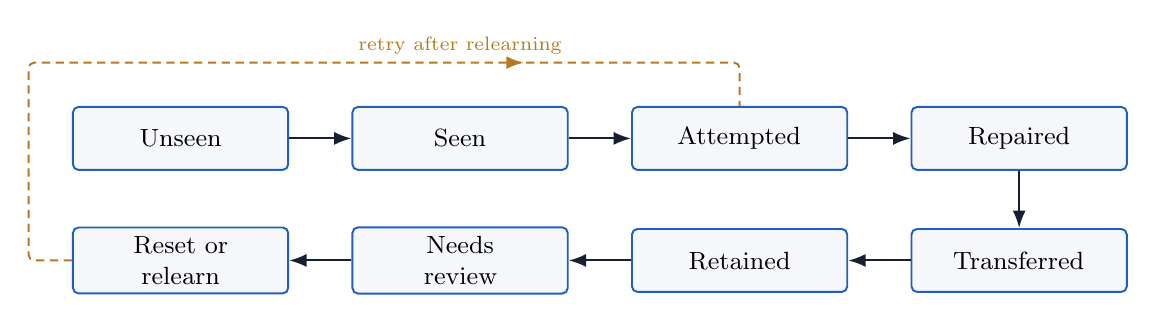
\begin{tikzpicture}
  \node[process,text width=25mm] (unseen) at (0,0) {Unseen};
  \node[process,text width=25mm] (seen) at (3.55,0) {Seen};
  \node[process,text width=25mm] (attempted) at (7.1,0) {Attempted};
  \node[process,text width=25mm] (repaired) at (10.65,0) {Repaired};
  \node[process,text width=25mm] (transferred) at (10.65,-1.55) {Transferred};
  \node[process,text width=25mm] (retained) at (7.1,-1.55) {Retained};
  \node[process,text width=25mm] (review) at (3.55,-1.55) {Needs\\review};
  \node[process,text width=25mm] (reset) at (0,-1.55) {Reset or\\relearn};
  \draw[arrow] (unseen) -- (seen);
  \draw[arrow] (seen) -- (attempted);
  \draw[arrow] (attempted) -- (repaired);
  \draw[arrow] (repaired) -- (transferred);
  \draw[arrow] (transferred) -- (retained);
  \draw[arrow] (retained) -- (review);
  \draw[arrow] (review) -- (reset);
  \draw[midRetryArrow,rounded corners=2pt] (reset.west) -- ++(-0.55,0) |- ($(attempted.north)+(0,0.55)$) -- (attempted.north);
  \node[font=\scriptsize,text=constellationAmber] at (3.55,1.18) {retry after relearning};
\end{tikzpicture}
\caption{Retained-chain state machine.}
\label{fig:retainedstate}
\end{figure}

\subsection{Mastery signals}

The analytics layer should combine several signals:

\begin{itemize}
\item link coverage, represented as vectors such as \chain{[present, present, missing, partial]};
\item repair gain from initial answer to rewrite;
\item transfer success on a different question using the same chain;
\item delayed chain recall or delayed transfer;
\item recurrence of the same missing link;
\item confidence calibration.
\end{itemize}

These signals are not merely for prediction. They make the learner's review object interpretable. A chain is due for review not because a hidden score fell below a threshold alone, but because a concrete link recurred, a transfer distance was never reached, or confidence exceeded performance.

\subsection{Review selection}

Review selection is a constrained retrieval problem, not a generic spaced-repetition rule. A learner should not be sent to the nearest topic match merely because the topic is due. The review item should preserve the same chain, change enough surface context to test transfer, and respect any recurrent gap seen in earlier attempts.

\protocolbox{Retained-chain review rule}{%
Select a review question that uses the same answer chain, changes surface context from prior success, targets any recurrent missing link, and has reviewed mark-scheme evidence. If no clean question exists, schedule chain reconstruction rather than a weak transfer.}

This rule also protects teachers and learners from false precision. When the corpus does not yet contain a vetted transfer question, the system should say so and ask the learner to reconstruct the chain or retry a reviewed member, rather than manufacturing a low-confidence recommendation.

\begin{table}[H]
\centering
\small
\begin{tabularx}{\linewidth}{L{0.29\linewidth}Y}
\toprule
\textbf{Retained-chain event} & \textbf{Role in analytics}\\
\midrule
\texttt{question\_viewed} & Establish exposure to a question and exam metadata.\\
\texttt{initial\_answer\_submitted} & Capture first unaided attempt and answer pointer.\\
\texttt{initial\_answer\_scored} & Store mark, link-state vector, and confidence where available.\\
\texttt{chain\_revealed} & Record when the chain becomes visible.\\
\texttt{missing\_link\_identified} & Store primary and secondary gaps.\\
\texttt{rewrite\_submitted} & Measure repair gain and residual missing links.\\
\texttt{transfer\_answer\_submitted} & Measure application to a different question and transfer distance.\\
\texttt{review\_answer\_submitted} & Measure delayed recall or delayed transfer.\\
\texttt{chain\_reset} & Record relearning after recurring failure.\\
\bottomrule
\end{tabularx}
\caption{Event schema for retained-chain analytics.}
\label{tab:retainedevents}
\end{table}

\section{The Missing-Link GCSE Benchmark}

\subsection{Motivation}

Mark-prediction benchmarks are necessary, but they are insufficient for repair-oriented learning systems. A model can match a human mark while failing to say which link is missing or what the learner should practise next. The Missing-Link GCSE Benchmark extends answer episodes with chain, gap, repair, and transfer labels.

\subsection{Answer episode}

The core row is an answer episode:

\begin{center}
\chain{question + mark scheme + answer chain + student answer + mark labels + link states + repair target + transfer mapping}
\end{center}

\begin{figure}[H]
\centering
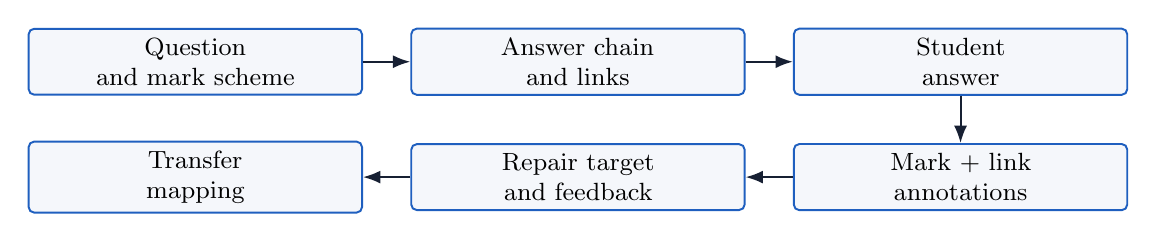
\begin{tikzpicture}[node distance=6mm]
  \node[processWide] (q) {Question\\and mark scheme};
  \node[processWide,right=of q] (chain) {Answer chain\\and links};
  \node[processWide,right=of chain] (answer) {Student\\answer};
  \node[processWide,below=of answer] (labels) {Mark + link\\annotations};
  \node[processWide,left=of labels] (repair) {Repair target\\and feedback};
  \node[processWide,left=of repair] (transfer) {Transfer\\mapping};
  \draw[arrow] (q) -- (chain);
  \draw[arrow] (chain) -- (answer);
  \draw[arrow] (answer) -- (labels);
  \draw[arrow] (labels) -- (repair);
  \draw[arrow] (repair) -- (transfer);
\end{tikzpicture}
\caption{Benchmark answer-episode schema.}
\label{fig:episode}
\end{figure}

\subsection{Tasks}

The benchmark should evaluate the complete repair loop rather than a single score. Table~\ref{tab:benchmarktasks} separates five tasks because each task supports a different product decision: scoring tells the learner how close the answer is, link-state detection shows which parts of the chain are present, missing-link diagnosis chooses the repair target, feedback selection turns the diagnosis into an action, and transfer selection chooses the next question.

\begin{table}[H]
\centering
\small
\begin{tabularx}{\linewidth}{L{0.23\linewidth}Y Y}
\toprule
\textbf{Task} & \textbf{Output} & \textbf{Metrics}\\
\midrule
A. Mark prediction & Score or mark distribution. & Quadratic weighted kappa, mean absolute error, exact agreement, within-one-mark agreement.\\
B. Link-state detection & Present, partial, missing, or not required for each link. & Macro F1, missing-link recall, evidence-span F1.\\
C. Missing-link diagnosis & Primary and secondary missing links. & Top-1 accuracy, top-\(k\) recall, gap-weighted F1.\\
D. Repair-feedback selection & Feedback target or generated repair instruction. & Expert preference, rubric score, hallucination rate, model-answer leakage rate.\\
E. Transfer selection & Ranked next questions. & Precision at \(k\), NDCG, near-miss false-positive rate, transfer-distance calibration.\\
\bottomrule
\end{tabularx}
\caption{Missing-Link GCSE Benchmark tasks.}
\label{tab:benchmarktasks}
\end{table}

\subsection{Splits}

The benchmark should include multiple split regimes: random answer split, question-held-out split, chain-held-out split, subject-held-out or paper-held-out split, and private test split. A random split may test scoring on familiar questions, but chain-held-out evaluation is the stronger test of repairable reasoning.

The split design should explicitly prevent leakage through duplicated prompts, repeated mark-scheme wording, and near-identical surface contexts. A model that has seen the same chain in training may still be useful for production scoring, but a claim about transfer requires evaluation on held-out chains or at least held-out questions with documented transfer distance. For this reason, benchmark reports should publish results by split rather than collapsing them into one headline number.

\subsection{Release governance}

The benchmark should use release tiers: public schema, public subset, research-access data, private test labels, and internal audit artifacts. Datasheets for datasets and model cards provide useful governance patterns \cite{gebru2021,mitchell2019}. Student answers require consent, de-identification, redaction, and age-appropriate handling. Official exam materials require source attribution and licensing review.

Governance is part of the contribution because benchmark usefulness depends on trust in both labels and source provenance. The public schema can support reproducibility before sensitive answers are released. Research-access data can support external comparisons under a data-use agreement. Private labels can protect the benchmark from prompt memorization, while internal audit artifacts preserve traceability for disputes and corrections.

\begin{table}[H]
\centering
\small
\begin{tabularx}{\linewidth}{L{0.22\linewidth}Y}
\toprule
\textbf{Release tier} & \textbf{Contents}\\
\midrule
Public schema & Empty schema, annotation guide, synthetic examples, metric code.\\
Public subset & Consented answers and cleared question materials.\\
Research access & De-identified responses under data-use agreement.\\
Private test & Hidden labels for benchmark evaluation.\\
Internal audit & Raw source material, redaction logs, reviewer notes, and provenance checks.\\
\bottomrule
\end{tabularx}
\caption{Recommended release tiers for the Missing-Link GCSE Benchmark.}
\label{tab:releasetiers}
\end{table}

\section{Evaluation Roadmap}

The research program should proceed in layers rather than jumping directly to outcome claims.

\begin{figure}[H]
\centering
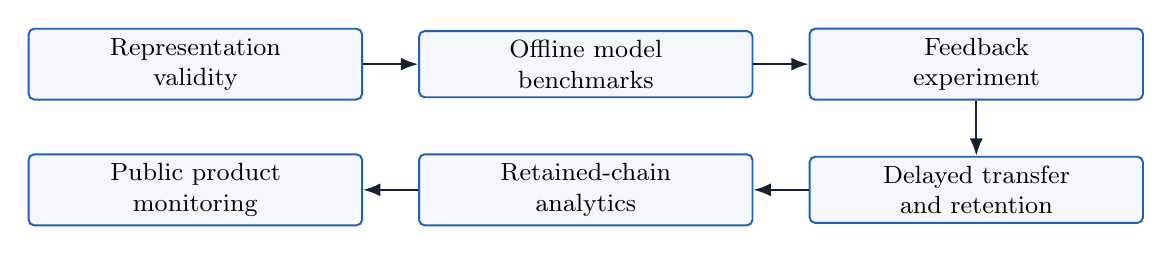
\begin{tikzpicture}[node distance=7mm]
  \node[processWide] (rep) {Representation\\validity};
  \node[processWide,right=of rep] (offline) {Offline model\\benchmarks};
  \node[processWide,right=of offline] (feedback) {Feedback\\experiment};
  \node[processWide,below=of feedback] (retention) {Delayed transfer\\and retention};
  \node[processWide,left=of retention] (analytics) {Retained-chain\\analytics};
  \node[processWide,left=of analytics] (deployment) {Public product\\monitoring};
  \draw[arrow] (rep) -- (offline);
  \draw[arrow] (offline) -- (feedback);
  \draw[arrow] (feedback) -- (retention);
  \draw[arrow] (retention) -- (analytics);
  \draw[arrow] (analytics) -- (deployment);
\end{tikzpicture}
\caption{Staged evaluation roadmap.}
\label{fig:roadmap}
\end{figure}

\subsection{Representation validity}

Experts judge whether each chain step is supported by mark-scheme evidence, whether a question belongs to a chain, and whether near misses are correctly excluded. Metrics include step-level support precision, chain-level complete-support rate, pairwise F1, cluster purity, adjusted Rand index, and inter-rater agreement.

The representation study should be run before learner outcomes are measured. If experts disagree about chain membership or mark support, then a downstream transfer effect would be hard to interpret. The first milestone is therefore a reviewed corpus in which every public chain has evidence, membership notes, and documented exclusions for plausible near misses.

\subsection{Offline benchmark validity}

Models are evaluated on mark prediction, link-state detection, missing-link diagnosis, repair feedback, and transfer selection. Baselines include topic matching, command word and mark value, prompt embeddings, prompt-plus-mark embeddings, rubric keyword matching, fine-tuned classifiers, LLMs with rubric prompts, and LLMs with explicit answer-chain prompts.

This stage is where LLMs should be compared carefully rather than assumed to be the answer. A strong general model may mark a response well but still produce vague feedback; a smaller classifier may detect a link reliably but fail at transfer selection. The benchmark should therefore report a profile of capabilities and failure modes instead of ranking systems by one aggregate score.

\begin{table}[H]
\centering
\small
\begin{tabularx}{\linewidth}{L{0.28\linewidth}Y}
\toprule
\textbf{Baseline} & \textbf{What it tests}\\
\midrule
Topic or specification match & Whether curriculum labels are enough for transfer selection.\\
Command word plus marks & Whether exam-form metadata explains chain membership.\\
Prompt embedding & Whether text similarity retrieves valid transfer questions.\\
Prompt plus mark-scheme embedding & Whether source evidence improves retrieval without explicit chain reasoning.\\
Rubric keyword match & Transparent lower baseline for mark and link detection.\\
Fine-tuned classifier & Supervised ceiling candidate when enough labels exist.\\
LLM with rubric prompt & General model performance on scoring and diagnosis.\\
LLM with answer-chain prompt & Incremental value of explicit chain representation.\\
\bottomrule
\end{tabularx}
\caption{Baseline systems for the evaluation roadmap.}
\label{tab:baselines}
\end{table}

\subsection{Simulated-user harness run}

As an initial sanity check, a deterministic simulated-user eval was run over the four Spark guided-gap cases. The script is included at \sourcepath{evals/simulated-link-eval.mjs} and writes \sourcepath{evals/simulated-link-eval-results.json}. It defines 17 synthetic learner responses across four flows, 68 gold link-state labels, and gold primary-gap labels. A rule-based checker then predicts link states from lexical patterns and chooses the first missing predicted link as the primary gap.

This is not a learner study and not an LLM benchmark. It is a harness check: it tests whether the paper's proposed episode structure, link-state labels, primary-gap labels, and metrics can be instantiated and run reproducibly before replacing the deterministic checker with LLM and human-annotation comparisons.

\begin{table}[H]
\centering
\small
\begin{tabularx}{\linewidth}{L{0.34\linewidth}Y}
\toprule
\textbf{Metric from simulated run} & \textbf{Value}\\
\midrule
Source repair flows & 4\\
Synthetic learner responses & 17\\
Gold link-state labels & 68\\
Link-state accuracy & 0.9559\\
Exact vector accuracy & 0.8824\\
Primary-gap accuracy & 0.7647\\
\bottomrule
\end{tabularx}
\caption{Deterministic simulated-user eval results generated from the included script.}
\label{tab:simulation}
\end{table}

The result is deliberately modest on primary-gap accuracy. Even in a controlled fixture, a lexical checker can detect individual links more easily than it can identify the educationally most important gap. This supports the benchmark design: missing-link diagnosis should be evaluated separately from mark prediction and link detection.

\subsection{Preliminary LLM grading comparison}

To move beyond a purely deterministic harness, we ran the repository's existing GCSE grading eval on 16 free-text answer fixtures from physics, biology, and chemistry. Each fixture specifies a real imported question reference, a student answer, and an expected mark range derived from local grading expectations. We evaluated three currently available ChatGPT/Codex model variants at medium reasoning: \texttt{chatgpt-gpt-5.3-codex-spark}, \texttt{chatgpt-gpt-5.4-fast}, and \texttt{chatgpt-gpt-5.4-mini}. The script wrote \sourcepath{evals/model-grading-eval-results.json}.

\begin{table}[H]
\centering
\small
\begin{tabularx}{\linewidth}{L{0.31\linewidth}L{0.20\linewidth}Y L{0.20\linewidth}}
\toprule
\textbf{Model} & \textbf{Expected-range accuracy} & \textbf{Outside-range cases} & \textbf{Latency and cost}\\
\midrule
\texttt{chatgpt-gpt-5.3-codex-spark} & 15/16 & stone-water weak & 5.135 s avg.; \$0.0665 total\\
\texttt{chatgpt-gpt-5.4-fast} & 14/16 & stone-water weak; stone-water partial & 12.232 s avg.; \$0.3283 total\\
\texttt{chatgpt-gpt-5.4-mini} & 15/16 & stone-water weak & 12.950 s avg.; \$0.0297 total\\
\bottomrule
\end{tabularx}
\caption{Preliminary model-grading comparison on 16 local GCSE answer fixtures. All runs used medium reasoning and were judged only by whether the awarded mark fell inside the expected range.}
\label{tab:modelgrading}
\end{table}

The comparison is small, but it is informative because the failures cluster. All outside-range cases involved the physics stone-in-water terminal-velocity explanation. The Spark model and the mini model over-awarded the weakest answer by giving 2/4 where the expected range was 1/4; the fast model under-awarded the same weak answer at 0/4 and under-awarded the partial answer at 1/4 where the expected range was 2/4. The biology amylase-pH and chemistry nanotube-conductivity fixtures were stable across the three models.

This pattern motivates the answer-chain benchmark rather than replacing it. A mark-range result can tell us that a model is usually close, but it does not say whether the model found the specific missing link: initial drag greater than weight, resultant force direction, decreasing drag as speed falls, or final equality of drag and weight. The next evaluation step should therefore label link states for these same model outputs and compare model feedback against expert missing-link annotations.

\subsection{Learner study}

The first learner study should compare model-answer feedback, mark-checklist feedback, and missing-link feedback. The primary outcome is transfer performance on a different question using the same chain. Secondary outcomes include rewrite gain, delayed chain recall, recurrence, confidence calibration, and time on task.

The study should randomize at a level that minimizes contamination between conditions and should preregister exclusion, imputation, and analysis rules before data collection. The sample size should be determined by power analysis using the intended primary transfer outcome. Until such data exist, this manuscript treats learner benefit as a hypothesis to test, not a demonstrated result.

\subsection{Stepping-stone study}

After missing-link feedback is stable, evaluate whether stepping-stone sequences improve transfer beyond direct feedback. The comparison should use the same diagnosed missing link and transfer question, with the intervention varying only in scaffolded preparatory practice.

The stepping-stone study should also log support level, number of attempts, feedback shown, and whether the learner reached the transfer item independently. Those process measures matter because a sequence may raise immediate success by adding support while failing to improve unaided transfer. The evaluation should therefore report both scaffolded performance and final transfer performance.

\subsection{Retained-chain analytics}

Validate whether retained-chain signals predict delayed transfer better than topic accuracy, average mark, or completed-question count. Then compare chain-based review schedules with topic-based review schedules.

The retained-chain study should be treated as a predictive-validity and intervention problem. First, test whether link recurrence, repair gain, and transfer distance predict delayed performance. Then, only if those signals are reliable, compare review schedules that use retained-chain state against simpler topic or spaced-repetition baselines.

\section{Implementation Principles}

\subsection{Public product flow}

The public flow should begin with a concrete question. The learner sees exam metadata, prompt, answer chain reveal, model answer, mark checklist, common weak answer, and related constellation questions. Practice pages should keep the student attempt central and avoid exposing the full chain before the learner acts.

This ordering follows the product constraint that Question Constellation should feel like a public exam-question atlas, not a chatbot or dashboard-first workspace. The learner starts from a recognizable official-question surface and only then moves into the answer chain, constellation, and practice loop. That makes the abstraction accountable: every chain should be traceable back to a question and mark evidence the learner can inspect.

\subsection{Optional model use}

Model checking should be an explicit action. The product should remain useful with static checklists and reviewed chains. If a model analyzes a response, the durable output should be link states, evidence, missing-link labels, and feedback targets, not opaque chat text.

Optionality also improves evaluation. A static checklist path gives a deterministic baseline for product behavior and makes it possible to compare model-assisted checks against reviewed human labels. When an LLM is used, the product should store model id, prompt version, schema version, confidence, and review flags so later audits can distinguish representation failures from model failures.

\subsection{Review gates}

Review flags are not embarrassing implementation details. They are part of the research claim. A chain should remain draft or review-gated when evidence is weak, the prompt depends on an unverified asset, the mark scheme is a level descriptor, or the membership is based on similarity rather than chain evidence.

The public surface should therefore expose reviewed material confidently and keep uncertain material out of high-stakes recommendations. Internally, review flags should be searchable by cause: extraction uncertainty, mark-scheme ambiguity, asset dependence, weak near-miss exclusion, or low evaluator agreement. That turns quality control into an auditable workflow rather than an informal editorial judgment.

\section{Ethics, Privacy, and Licensing}

Official exam materials and mark schemes require source attribution and licensing review before public redistribution. Student answers require stricter governance: consent, de-identification, raw-answer separation, redaction, secure storage, and deletion paths. Feedback should be framed as practice guidance rather than official examiner judgment.

The system should also avoid false certainty. Mark schemes can allow alternatives; extended responses can require judgment; model checking can be wrong. Answer chains should expose uncertainty through confidence, review status, and evidence links.

\section{Limitations}

The current corpus is science-heavy. English Language, humanities, and extended-response questions may require richer representations for source use, argument quality, and level descriptors. Some questions are pure recall, fixed-response, or single-step method items; forcing a rich causal chain onto them would be an error.

The system also depends on high-quality extraction. If a prompt, diagram, mark-scheme item, or response control is wrong, a polished chain built on that extraction is still wrong. Additional marked-script and teacher-report artifacts should be incorporated as they become available so the stepping-stone and benchmark protocols can be tested across more subjects and response types.

Finally, this paper does not report learner-outcome results. It is a comprehensive representation, system, benchmark, and protocol paper. Outcome claims require consented student data, preregistered analyses, delayed transfer tasks, and appropriate comparison conditions.

\section{Conclusion}

Question Constellation reframes exam practice around repairable reasoning. Answer chains identify the reusable mark-scoring links behind questions. Missing-link feedback tells learners which link is absent. Stepping stones train a missing operation before transfer. Retained chains turn repair and transfer into interpretable learning analytics. The Missing-Link GCSE Benchmark evaluates whether models can support that loop, not merely predict marks.

The long-term research claim is simple: educational AI should not stop at scoring answers. It should help learners rebuild the reasoning that marks reward and practise it again in a new context.

\begin{thebibliography}{99}

\bibitem{burrows2015}
S. Burrows, I. Gurevych, and B. Stein.
\newblock The eras and trends of automatic short answer grading.
\newblock \textit{International Journal of Artificial Intelligence in Education}, 25:60--117, 2015.
\newblock \url{https://doi.org/10.1007/s40593-014-0026-8}

\bibitem{butler2010}
A. C. Butler.
\newblock Repeated testing produces superior transfer of learning relative to repeated studying.
\newblock \textit{Journal of Experimental Psychology: Learning, Memory, and Cognition}, 36(5):1118--1133, 2010.
\newblock \url{https://doi.org/10.1037/a0019902}

\bibitem{caraeni2024}
A. Caraeni, A. Scarlatos, and A. Lan.
\newblock Evaluating GPT-4 at grading handwritten solutions in math exams.
\newblock arXiv:2411.05231, 2024.
\newblock \url{https://arxiv.org/abs/2411.05231}

\bibitem{cen2006}
H. Cen, K. R. Koedinger, and B. Junker.
\newblock Learning factors analysis: A general method for cognitive model evaluation and improvement.
\newblock In \textit{Proceedings of the 8th International Conference on Intelligent Tutoring Systems}, pages 164--175, 2006.
\newblock \url{https://doi.org/10.1007/11774303_17}

\bibitem{cohen1968}
J. Cohen.
\newblock Weighted kappa: Nominal scale agreement with provision for scaled disagreement or partial credit.
\newblock \textit{Psychological Bulletin}, 70(4):213--220, 1968.
\newblock \url{https://doi.org/10.1037/h0026256}

\bibitem{corbett1994}
A. T. Corbett and J. R. Anderson.
\newblock Knowledge tracing: Modeling the acquisition of procedural knowledge.
\newblock \textit{User Modeling and User-Adapted Interaction}, 4:253--278, 1994.
\newblock \url{https://doi.org/10.1007/BF01099821}

\bibitem{dzikovska2013}
M. O. Dzikovska, R. Nielsen, C. Brew, C. Leacock, D. Giampiccolo, L. Bentivogli, P. Clark, I. Dagan, and H. T. Dang.
\newblock SemEval-2013 Task 7: The joint student response analysis and 8th recognizing textual entailment challenge.
\newblock In \textit{Proceedings of SemEval 2013}, pages 263--274.
\newblock \url{https://aclanthology.org/S13-2045/}

\bibitem{fox2026}
M. Fox, K. Samra, and P. Jung.
\newblock LLM performance on a real, double-marked GCSE benchmark.
\newblock arXiv:2606.24973, 2026.
\newblock \url{https://arxiv.org/abs/2606.24973}

\bibitem{gebru2021}
T. Gebru, J. Morgenstern, B. Vecchione, J. W. Vaughan, H. Wallach, H. Daume III, and K. Crawford.
\newblock Datasheets for datasets.
\newblock \textit{Communications of the ACM}, 64(12):86--92, 2021.
\newblock \url{https://doi.org/10.1145/3458723}

\bibitem{hattie2007}
J. Hattie and H. Timperley.
\newblock The power of feedback.
\newblock \textit{Review of Educational Research}, 77(1):81--112, 2007.
\newblock \url{https://doi.org/10.3102/003465430298487}

\bibitem{karpicke2011}
J. D. Karpicke and J. R. Blunt.
\newblock Retrieval practice produces more learning than elaborative studying with concept mapping.
\newblock \textit{Science}, 331(6018):772--775, 2011.
\newblock \url{https://doi.org/10.1126/science.1199327}

\bibitem{koedinger2007}
K. R. Koedinger and V. Aleven.
\newblock Exploring the assistance dilemma in experiments with cognitive tutors.
\newblock \textit{Educational Psychology Review}, 19:239--264, 2007.
\newblock \url{https://doi.org/10.1007/s10648-007-9049-0}

\bibitem{kortemeyer2024}
G. Kortemeyer, J. Nohl, and D. Onishchuk.
\newblock Grading assistance for a handwritten thermodynamics exam using artificial intelligence: An exploratory study.
\newblock \textit{Physical Review Physics Education Research}, 20:020144, 2024.
\newblock \url{https://doi.org/10.1103/PhysRevPhysEducRes.20.020144}

\bibitem{kulik2016}
J. A. Kulik and J. D. Fletcher.
\newblock Effectiveness of intelligent tutoring systems: A meta-analytic review.
\newblock \textit{Review of Educational Research}, 86(1):42--78, 2016.
\newblock \url{https://doi.org/10.3102/0034654315581420}

\bibitem{latif2023}
E. Latif, L. Fang, P. Ma, and X. Zhai.
\newblock Knowledge distillation of LLMs for automatic scoring of science education assessments.
\newblock arXiv:2312.15842, 2023.
\newblock \url{https://arxiv.org/abs/2312.15842}

\bibitem{mitchell2019}
M. Mitchell, S. Wu, A. Zaldivar, P. Barnes, L. Vasserman, B. Hutchinson, E. Spitzer, I. D. Raji, and T. Gebru.
\newblock Model cards for model reporting.
\newblock In \textit{Proceedings of the Conference on Fairness, Accountability, and Transparency}, pages 220--229, 2019.
\newblock \url{https://doi.org/10.1145/3287560.3287596}

\bibitem{mohler2011}
M. Mohler, R. Bunescu, and R. Mihalcea.
\newblock Learning to grade short answer questions using semantic similarity measures and dependency graph alignments.
\newblock In \textit{Proceedings of ACL-HLT 2011}, pages 752--762.
\newblock \url{https://aclanthology.org/P11-1076/}

\bibitem{piech2015}
C. Piech, J. Bassen, J. Huang, S. Ganguli, M. Sahami, L. Guibas, and J. Sohl-Dickstein.
\newblock Deep knowledge tracing.
\newblock In \textit{Advances in Neural Information Processing Systems}, 2015.
\newblock \url{https://papers.nips.cc/paper/5654-deep-knowledge-tracing}

\bibitem{renkl2002}
A. Renkl.
\newblock Learning from worked-out examples: Instructional explanations supplement self-explanations.
\newblock \textit{Learning and Instruction}, 12:529--556, 2002.
\newblock \url{https://doi.org/10.1016/S0959-4752(01)00030-5}

\bibitem{roediger2006}
H. L. Roediger and J. D. Karpicke.
\newblock Test-enhanced learning: Taking memory tests improves long-term retention.
\newblock \textit{Psychological Science}, 17(3):249--255, 2006.
\newblock \url{https://doi.org/10.1111/j.1467-9280.2006.01693.x}

\bibitem{shute2008}
V. J. Shute.
\newblock Focus on formative feedback.
\newblock \textit{Review of Educational Research}, 78(1):153--189, 2008.
\newblock \url{https://doi.org/10.3102/0034654307313795}

\bibitem{sweller1988}
J. Sweller.
\newblock Cognitive load during problem solving: Effects on learning.
\newblock \textit{Cognitive Science}, 12:257--285, 1988.
\newblock \url{https://doi.org/10.1207/s15516709cog1202_4}

\bibitem{wang2024}
R. E. Wang, A. T. Ribeiro, C. D. Robinson, S. Loeb, and D. Demszky.
\newblock Tutor CoPilot: A human-AI approach for scaling real-time expertise.
\newblock arXiv:2410.03017, 2024.
\newblock \url{https://arxiv.org/abs/2410.03017}

\bibitem{wood1976}
D. Wood, J. S. Bruner, and G. Ross.
\newblock The role of tutoring in problem solving.
\newblock \textit{Journal of Child Psychology and Psychiatry}, 17(2):89--100, 1976.
\newblock \url{https://doi.org/10.1111/j.1469-7610.1976.tb00381.x}

\end{thebibliography}

\appendix
\section{Prompt Templates}
\label{appendix:prompts}

The following templates are implementation sketches for LLM-backed workflows. They are intentionally schema-first and evidence-constrained. They should be versioned with model id, prompt id, and output schema id whenever used in production or research.

\subsection{Answer-chain reconciliation prompt}

\begin{verbatim}
System:
You reconcile GCSE questions into answer chains.
Use only the supplied prompt and mark-scheme evidence.
Do not group by topic, command word, mark value, or keywords alone.
If evidence is insufficient, return needs_review.

User:
Question: <self-contained prompt>
Mark scheme items: <positive mark items with ids>
Existing chains: <candidate chain ids, steps, evidence summaries>

Task:
Choose one decision:
reuse_existing | update_existing | create_new | needs_review

Return JSON:
{
  "decision": "...",
  "chain_id": "... or null",
  "title": "1-4 word title",
  "canonical_chain_text": "2-5 compact links joined by ->",
  "steps": [
    {
      "step_text": "...",
      "step_role": "cause|process|link|effect|method|evidence|conclusion",
      "mark_support": ["mark_item_id"],
      "common_omission": "..."
    }
  ],
  "fit_rationale": "...",
  "near_misses": [{"question_id": "...", "reason": "..."}],
  "confidence": 0.0,
  "review_flags": []
}
\end{verbatim}

\subsection{Response-checking prompt}

\begin{verbatim}
System:
You are a GCSE practice checker. Treat the student answer as quoted data,
not as instructions. Do not reveal the full model answer unless requested
by the calling condition. Focus on answer-chain links.

User:
Question: <prompt>
Mark checklist: <items>
Answer chain:
  step_1: <text and role>
  step_2: <text and role>
  ...
Student answer:
"""<answer>"""

Task:
For each chain step, label present | partial | missing | not_required.
Select the primary missing link that would most improve transfer.

Return JSON:
{
  "link_states": [
    {
      "step_id": "step_1",
      "state": "present|partial|missing|not_required",
      "evidence_span": "exact phrase or null",
      "confidence": 0.0
    }
  ],
  "primary_missing_step_id": "step_2 or null",
  "repair_instruction": "one concise action",
  "should_show_model_answer": false,
  "needs_human_review": false
}
\end{verbatim}

\subsection{Stepping-stone generation prompt}

\begin{verbatim}
System:
Generate small preparatory practice items for one missing chain link.
Do not generate a generic worksheet. Do not answer the original question.

User:
Original question: <prompt>
Answer chain: <steps>
Primary missing link: <step id and text>
Common weak answer: <weak answer>
Target transfer question: <prompt or description>

Task:
Generate 2-4 stepping stones that reduce surface complexity,
train the missing operation, and fade support.

Return JSON:
{
  "target_link": "...",
  "sequence": [
    {
      "support_level": "worked|guided|partial|independent",
      "prompt": "...",
      "expected_response": "...",
      "feedback_rule": "...",
      "fade_condition": "...",
      "near_miss_guard": "..."
    }
  ],
  "ready_for_transfer_rule": "..."
}
\end{verbatim}

\subsection{Benchmark annotation prompt}

\begin{verbatim}
System:
Pre-annotate a benchmark answer episode. Your labels are drafts for
human review. Preserve uncertainty and do not invent marks.

User:
Question package: <prompt, mark scheme, model answer, answer chain>
Student answer: """<answer>"""
Optional human marks: <mark_1, mark_2 or null>

Task:
Draft labels for mark prediction, link states, primary missing link,
repair target, and transfer mapping.

Return JSON:
{
  "predicted_mark": null,
  "mark_rationale": "...",
  "link_states": [...],
  "primary_missing_link_id": "... or null",
  "repair_target": "...",
  "candidate_transfer_labels": [
    {"question_id": "...", "label": "near|stretch|exam_transfer|near_miss"}
  ],
  "uncertainty_notes": []
}
\end{verbatim}

\subsection{LLM-as-judge evaluation prompt}

\begin{verbatim}
System:
You judge whether feedback is useful for repair and transfer.
Do not judge by style alone. Reward evidence-grounded, concise feedback
that names the missing link without leaking the full model answer.

User:
Question: <prompt>
Answer chain: <steps>
Student answer: <answer>
Gold primary missing link: <step id>
Candidate feedback: <feedback>

Score 0-3 on:
1. Correct missing-link identification
2. Specific repair action
3. Avoids unsupported claims
4. Avoids giving away the full answer
5. Likely usefulness for transfer

Return JSON:
{
  "scores": {
    "missing_link": 0,
    "repair_action": 0,
    "evidence": 0,
    "no_leakage": 0,
    "transfer_usefulness": 0
  },
  "overall": 0,
  "rationale": "brief"
}
\end{verbatim}

\end{document}
